\documentclass[a4paper, 11pt]{article}

%% Fonts and Typography
\usepackage{beramono}
\usepackage{titlesec}
% SECTION: bold, compact
\titleformat{\section}
  {\large\bfseries}
  {\thesection}{0.6em}{}

\titlespacing*{\section}{0pt}{0.9\baselineskip}{0.4\baselineskip}

% SUBSECTION: bold, compact
\titleformat{\subsection}
  {\normalsize\bfseries}
  {\thesubsection}{0.6em}{}

\titlespacing*{\subsection}{0pt}{0.6\baselineskip}{0.3\baselineskip}

% SUBSUBSECTION: bold italic, compact
\titleformat{\subsubsection}
  {\small\bfseries\itshape}
  {\thesubsubsection}{0.6em}{}

\titlespacing*{\subsubsection}{0pt}{0.5\baselineskip}{0.2\baselineskip}
\usepackage{amsmath, amssymb}
\usepackage{setspace}

%% Graphics and Colors
\usepackage{graphicx} 
\graphicspath{ {figures/}{Billeder/} }
\usepackage{tikz}
\usetikzlibrary{arrows.meta, positioning, shapes.geometric, decorations.pathmorphing, calc, patterns}
\usepackage{color, colortbl}

%% Tables and Floats
\usepackage{floatrow}
\newfloatcommand{capbtabbox}{table}[][\FBwidth]
\usepackage{booktabs}
\usepackage{tabularx}

% Hyperref setup
\usepackage[hidelinks]{hyperref}
\definecolor{LinkBlue}{HTML}{3B6EA8}   % muted blue
\definecolor{CiteGreen}{HTML}{2F8F6B}  % muted green
\definecolor{UrlPurple}{HTML}{7A5EA8}  % muted purple

\hypersetup{
  unicode=true,
  colorlinks=true,
  linkcolor=LinkBlue,     % internal links (sections, equations, figures, toc)
  citecolor=CiteGreen,    % citations
  urlcolor=UrlPurple,     % urls
  filecolor=UrlPurple,    % local file links (rare)
  menucolor=LinkBlue,
}
\usepackage{pdfpages}
\usepackage{url}

%% Code Listings
\usepackage{soul}

% Table float box with bottom caption, box width adjusted to content
\usepackage{forest}

%% Miscellaneous
\usepackage{blindtext}
\usepackage{circuitikz}
\usepackage{subfiles}
\usepackage{adjustbox}
\usepackage{fancyhdr}
\usepackage{lastpage}
\usepackage{soul}
\usepackage{wrapfig}
\usepackage{booktabs}
\usepackage{subcaption}
\usepackage{float}

%% Custom Commands and Environments
\makeatletter
\renewcommand*\env@matrix[1][*\c@MaxMatrixCols c]{%
   \hskip -\arraycolsep
   \let\@ifnextchar\new@ifnextchar
   \array{#1}}
\makeatother

%% Matematik og kode formatering
\usepackage{physics}
\usepackage{amsmath}
\usepackage{minted}
\usepackage[dvipsnames]{xcolor}
\setminted{
    frame=lines,
    framesep=2mm,
    baselinestretch=1.2,
    fontsize=\small,
    linenos,
    numbersep=5pt,
    xleftmargin=10pt,
    tabsize=2,
    breaklines=true,
    breakanywhere=true,
    style=tango
}



% new
\usepackage{siunitx}
\usepackage[table]{xcolor}
\usepackage{makecell}
\usepackage{caption}
\usepackage{booktabs}
\usepackage{makecell}
\usepackage{siunitx}
\usepackage{rotating}
\usepackage{caption}


\sisetup{
  round-mode = places,
  round-precision = 2,
  retain-explicit-plus = true,
  detect-weight = true,
  detect-inline-weight = math
}
\newcommand{\pos}[1]{\textcolor{teal!70!black}{+#1}}
\renewcommand{\neg}[1]{\textcolor{red!75!black}{#1}}



%% Basic Document Settings
\usepackage[T1]{fontenc}
\usepackage[utf8]{inputenc}
\usepackage[english]{babel}
\usepackage[top=2.5cm,bottom=2.5cm,left=1.8cm,right=1.8cm]{geometry}
\usepackage{parskip}
\usepackage{xcolor}
\usepackage{newpxmath}
%% \usepackage{newpxtext}
\usepackage{graphicx}
\pagestyle{fancy}
\fancyhf{}
\renewcommand{\footrulewidth}{0.4pt}
\linespread{1}

%% BIBLIOGRAPHY
\usepackage[
backend=biber,
style=ieee,
sorting=ynt
]{biblatex}
\addbibresource{references.bib}

%%%%%%%%%%%%%%%%%%%%%%%%%%%%%%%%%%%%%%%%%%%%%%%%%%%%%%%%%%%%%%%%%%%
%%%%%%%%%%%%%%%%%%%%%%%%%%%%%%%%%%%%%%%%%%%%%%%%%%%%%%%%%%%%%%%%%%%
%%%%%%%%%%%%%%%%%%%%%%%%%%%%%%%%%%%%%%%%%%%%%%%%%%%%%%%%%%%%%%%%%%%
%%%%%%%%%%%%%%%%%%%%%%%%%%%%%%%%%%%%%%%%%%%%%%%%%%%%%%%%%%%%%%%%%%%

%% HEADER / FOOTER Customization
\rhead{
\includegraphics[height=7.5mm]{Billeder/Danmarks_Tekniske_Universitet_(logo).svg.png}}
\lhead{{\scshape FermaCore: A Discrete-Event Simulation Study} - 42417}
\rfoot{Page \thepage\,/ \pageref{LastPage}}
\lfoot{\textit{Group 16 - Manufacturing - s224927, s224917}}

%%%%%%%%%%%%%%%%%%%%%%%%%%%%%%%%%%%%%%%%%%%%%%%%%%%%%%%%%%%%%%%%%%%
%%%%%%%%%%%%%%%%%%%%%%%%%%%%%%%%%%%%%%%%%%%%%%%%%%%%%%%%%%%%%%%%%%%
%%%%%%%%%%%%%%%%%%%%%%%%%%%%%%%%%%%%%%%%%%%%%%%%%%%%%%%%%%%%%%%%%%%
%%%%%%%%%%%%%%%%%%%%%%%%%%%%%%%%%%%%%%%%%%%%%%%%%%%%%%%%%%%%%%%%%%%


% =====================================================================
%  42417 Simulation in Operations Management -- Case Study Project
%  Manufacturing case: FermaCore Labs
%  HARD PAGE LIMIT: 15 pages INCLUDING the front page. Stay lean.
%  Report structure is fixed by the case brief -- do NOT reorder.
% =====================================================================

\begin{document}

\begin{titlepage}
  \thispagestyle{empty}

  %--- Top strip: Authors (left) + DTU logo (right)
  \noindent
   \begin{minipage}[t]{0.62\textwidth}
    \vspace{0pt}
    \raggedright
    \textbf{\large \textsc{Jacob Brams (s224927)}}\\[7pt]
    \textbf{\large \textsc{Gustav Maglehøj Hansen (s224917)}}\\[7pt]
    \textbf{\large \textsc{Group XX}}\\[7pt]
  \end{minipage}%
  \hfill
  \begin{minipage}[t]{0.35\textwidth}
    \vspace{0pt}
    \raggedleft
    
\includegraphics[height=50mm]{Billeder/Danmarks_Tekniske_Universitet_(logo).svg.png}
  \end{minipage}

  %--- Centered block (title + course info)
  \vspace*{-80mm}
  \vfill
  \begin{center}
    \noindent\rule{1\textwidth}{1pt}\\[12pt]
{\Huge\bfseries\scshape
\linespread{1.25}\selectfont
A Discrete-Event Simulation Study\\
of the FermaCore Tablet Line\par
}\vspace{10pt}
    {\Large \scshape Simulation in Operations Management}\\[8pt]
    June 2026 --- 42417\\[8pt]
    \textit{\today}\\[15pt]
    \noindent\rule{1\textwidth}{1pt}
  \end{center}
  \vfill

\end{titlepage}

\newpage
\setcounter{page}{0}
\tableofcontents
\newpage

% --- Section numbering follows the mandatory case structure ---
\section{Introduction and Objective}
\label{sec:intro}

FermaCore Labs operates a tablet production line combining batch-type and rate-based operations. Management's 2030 plan aims to maximize output within the existing capacity before committing to long-lead-time capital expansions. 

The objective of this study is to use discrete-event simulation (DES) in AnyLogic to map the current system dynamics and identify operational bottlenecks. Using this baseline, we quantify the effects of targeted improvements (equipment additions and batch resequencing) and stress-test the line against the intensifying 2030 demand schedule to locate the constraint that caps its output.

\subsection*{Scope}
This report covers the mandatory simulation requirements: evaluating the current baseline, finding the bottleneck, and stress-testing the line under the 2030 demand schedule. We also include one optional analysis on Industry 4.0, specifically predictive maintenance at the tablet press, where sensors reduce scrap by catching press drift before it goes out of specification.                 % Objective of the study
\section{Statement of Collaboration}
\label{sec:collab}

% Mandatory. List other groups you collaborated with, or state none.
We did not collaborate with any other group on this project.

The work was carried out jointly throughout. Both authors developed the
conceptual model and KPI set together and co-wrote the report.
\textsc{Jacob Brams} took lead responsibility for the input modelling, output
analysis and experimental design; \textsc{Gustav Maglehøj Hansen} took lead
responsibility for the AnyLogic implementation and verification.
         % Statement of collaboration
\section{Performance Management}
\label{sec:performance}

To evaluate the FermaCore line and to compare improvement scenarios, we track
five Key Performance Indicators (KPIs), described with the S.M.A.R.T.\ framework
against management's objectives. Four are primary and cover output (throughput),
the bottleneck (utilisation), congestion (flow time and WIP) and schedule
adherence (on-time delivery); one is secondary and covers material efficiency
(yield). Table~\ref{tab:kpis} gives the baseline value of each KPI, with the full
results in Sections~\ref{sec:output} and~\ref{sec:experiments}.

\begin{table}[H]
\centering
\caption{Performance metrics, S.M.A.R.T.\ justification and baseline value.}
\label{tab:kpis}
\renewcommand{\arraystretch}{1.2}%
\small
\begin{tabularx}{\textwidth}{@{} >{\raggedright\arraybackslash}p{3.5cm} X @{}}
\toprule
\rowcolor{black!5}
\textbf{Key Performance Indicator} & \multicolumn{1}{c}{\textbf{S.M.A.R.T.}} \\
\midrule

\textbf{Weekly throughput}\newline
\textcolor{gray}{\footnotesize Baseline: \num{60972} bottles} &
\textcolor{red!70!black}{\textbf{S:}} Bottles shipped from the packaging lines. \newline
\textcolor{orange!80!black}{\textbf{M:}} Counted at the sink via \texttt{bottlesShipped}. \newline
\textcolor{green!60!black}{\textbf{A:}} Baseline sets the ceiling; improvements are compared to it. \newline
\textcolor{blue!70!black}{\textbf{R:}} The output management wants to raise before any expansion. \newline
\textcolor{purple!70!black}{\textbf{T:}} Per terminating 50-batch run. \\
\midrule

\textbf{Station utilisation}\newline
\textcolor{gray}{\footnotesize Baseline: dryer \SI{94.9}{\percent} (binding)} &
\textcolor{red!70!black}{\textbf{S:}} Busy share of drying, cleaning team and packaging. \newline
\textcolor{orange!80!black}{\textbf{M:}} Busy hours over available hours, from the resource pools. \newline
\textcolor{green!60!black}{\textbf{A:}} Read directly from AnyLogic each run. \newline
\textcolor{blue!70!black}{\textbf{R:}} Locates the bottleneck and shows if a fix only shifts it. \newline
\textcolor{purple!70!black}{\textbf{T:}} Tracked across the whole run. \\
\midrule

\textbf{Flow time and WIP}\newline
\textcolor{gray}{\footnotesize Baseline: \SI{180}{h} / 19.5 batches} &
\textcolor{red!70!black}{\textbf{S:}} Time a batch spends in the line, and batches in process. \newline
\textcolor{orange!80!black}{\textbf{M:}} \texttt{meanFlowTime} and \texttt{avgWIP}, linked by Little's Law. \newline
\textcolor{green!60!black}{\textbf{A:}} Logged from agent entry and exit times. \newline
\textcolor{blue!70!black}{\textbf{R:}} Measures congestion and lead time as load grows toward 2030. \newline
\textcolor{purple!70!black}{\textbf{T:}} Per batch, and time-averaged over the run. \\
\midrule

\textbf{On-time delivery}\newline
\textcolor{gray}{\footnotesize Baseline: \SI{100}{\percent} (max dev.\ \SI{18.5}{h})} &
\textcolor{red!70!black}{\textbf{S:}} Share of batches shipped within one day of the planned date. \newline
\textcolor{orange!80!black}{\textbf{M:}} \texttt{releaseViolations} and \texttt{maxReleaseDev} against the \SI{24}{h} rule. \newline
\textcolor{green!60!black}{\textbf{A:}} Compared against the plan's release dates each run. \newline
\textcolor{blue!70!black}{\textbf{R:}} The case's one-day release constraint; tested under 2030 demand. \newline
\textcolor{purple!70!black}{\textbf{T:}} Per batch, summarised per run. \\
\midrule

\textbf{System yield}\newline
\textcolor{gray}{\footnotesize Secondary, baseline scrap \SI{6.2}{\percent}} &
\textcolor{red!70!black}{\textbf{S:}} Good tablets kept versus tablets scrapped. \newline
\textcolor{orange!80!black}{\textbf{M:}} \texttt{scrapRate} from premix, press and packaging losses. \newline
\textcolor{green!60!black}{\textbf{A:}} Computed from scrap events at the end of each run. \newline
\textcolor{blue!70!black}{\textbf{R:}} The lever behind Industry 4.0 (press scrap \SI{10}{\percent} to \SI{4}{\percent}). \newline
\textcolor{purple!70!black}{\textbf{T:}} Cumulative per terminating run. \\

\bottomrule
\end{tabularx}
\end{table}
           % KPIs + rationale
\section{Modelling}
\label{sec:conceptual}

One process-batch flows as a single agent through six operations, becoming a
specific product only at coating. The plan gives each batch as
\SI{150}{\kilo\gram} of active-ingredient powder blend; \SI{75}{\kilo\gram} of
excipients is added in premix, giving a \SI{225}{\kilo\gram} batch of
\num{300000} tablets.
Figure~\ref{fig:flow} is the high-level flow chart; Figure~\ref{fig:activity} is
the activity diagram in Rossetti notation~\cite{rossetti2016}, laid out as a
left-to-right flow that wraps across rows. Circles are queues, rectangles are
activities with their delay distribution, and small circles are resources. Each
resource use is marked with a striped half-moon for the seize and a solid
half-moon for the release. Premix is drawn as its two physical units (old and
new), which differ in speed and failure rate; identical parallel resources
(presses, packaging lines) are kept as one block with a capacity count.

\subsection{System flow chart}
\label{sec:flow}
\begin{figure}[H]
\centering
\resizebox{0.40\textwidth}{!}{%
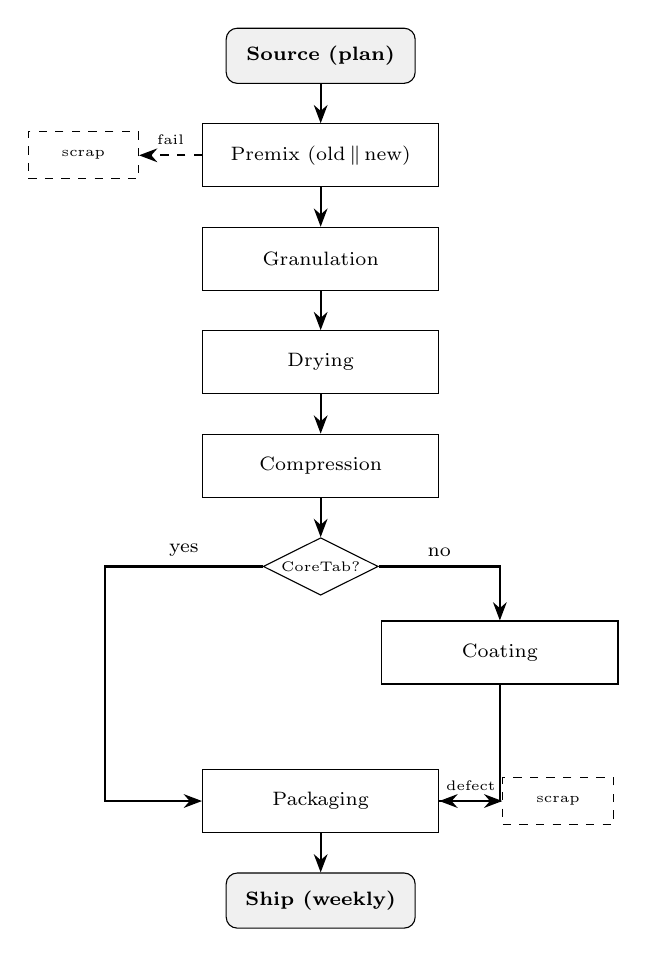
\begin{tikzpicture}[
  >=Stealth, font=\scriptsize, node distance = 5mm and 8mm,
  pr/.style={rectangle, draw, align=center, minimum width=30mm, minimum height=8mm},
  tm/.style={rectangle, draw, rounded corners=4pt, fill=black!6, align=center, minimum width=24mm, minimum height=7mm, font=\scriptsize\bfseries},
  dd/.style={diamond, draw, aspect=2, align=center, font=\tiny, inner sep=1pt},
  sc/.style={rectangle, draw, dashed, align=center, font=\tiny, minimum width=14mm, minimum height=6mm},
  a/.style={->, thick}]
\node[tm] (s) {Source (plan)};
\node[pr, below=of s] (pm) {Premix (old\,$\parallel$\,new)};
\node[pr, below=of pm] (gr) {Granulation};
\node[pr, below=of gr] (dr) {Drying};
\node[pr, below=of dr] (cp) {Compression};
\node[dd, below=of cp] (cd) {CoreTab?};
\node[pr, below right=5mm and 4mm of cd] (ct) {Coating};
\node[pr, below=22mm of cd] (pk) {Packaging};
\node[tm, below=of pk] (sh) {Ship (weekly)};
\node[sc, left=8mm of pm] (sp) {scrap};
\node[sc, right=8mm of pk] (sp2) {scrap};
\draw[a](s)--(pm);\draw[a](pm)--(gr);\draw[a](gr)--(dr);\draw[a](dr)--(cp);\draw[a](cp)--(cd);
\draw[a](cd.east)-|(ct.north) node[pos=.25,above]{no};
\draw[a](ct)|-(pk.east);
\draw[a](cd.west)--++(-20mm,0) node[pos=.5,above]{yes} |-(pk.west);
\draw[a](pk)--(sh);
\draw[a,dashed](pm)--(sp) node[pos=.5,above,font=\tiny]{fail};
\draw[a,dashed](pk)--(sp2) node[pos=.5,above,font=\tiny]{defect};
\end{tikzpicture}%
}
\caption{Simple flow chart of the FermaCore line. CoreTab skips coating; a premix
failure or pre-packaging inspection scraps material.}
\label{fig:flow}
\end{figure}

\subsection{Activity diagram}
\label{sec:activity}
\begin{figure}[H]
\centering
% Changed from \textwidth to 0.75\textwidth to reduce physical size
\resizebox{0.75\textwidth}{!}{%
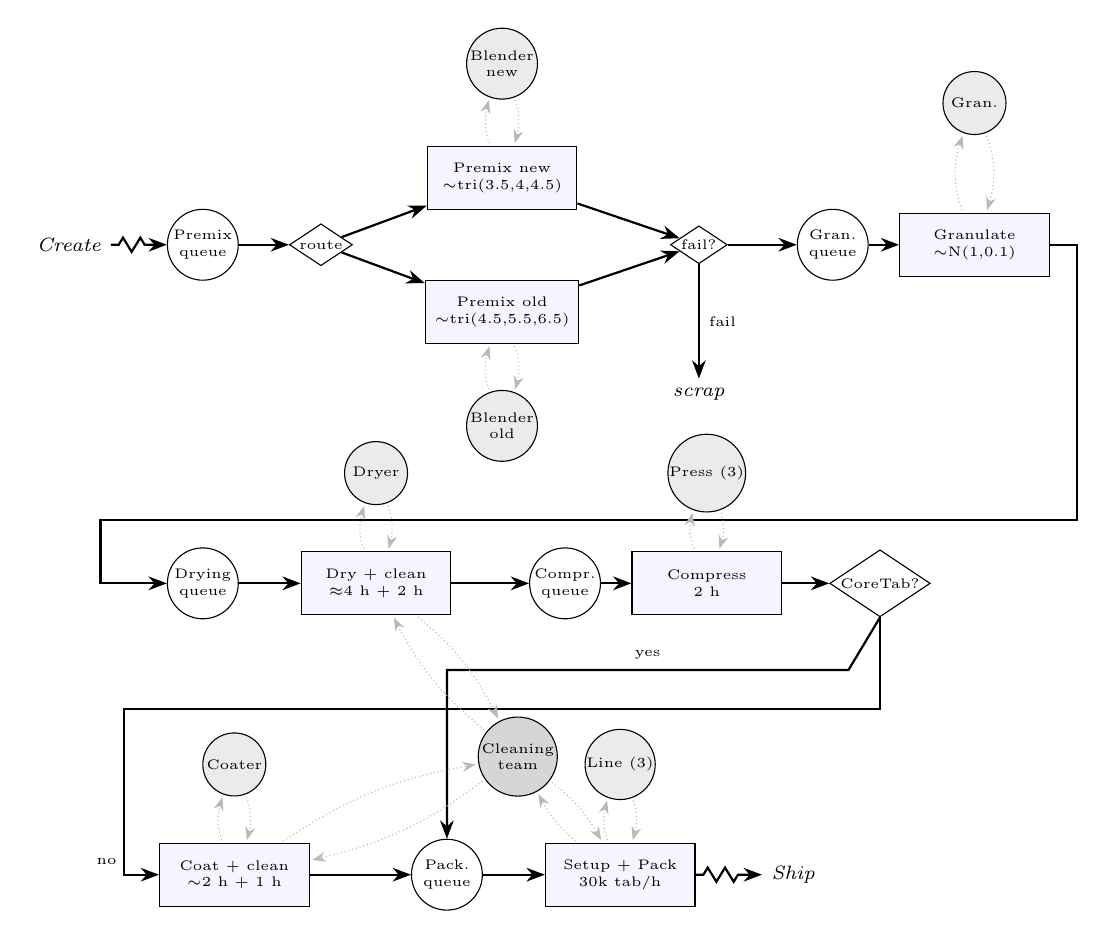
\begin{tikzpicture}[
  >=Stealth, font=\scriptsize,
  qu/.style={circle, draw, align=center, minimum size=9mm, inner sep=0.3pt, font=\tiny},
  ac/.style={rectangle, draw, fill=blue!4, align=center, minimum height=8mm, minimum width=19mm, font=\tiny},
  rs/.style={circle, draw, fill=black!8, align=center, minimum size=8mm, inner sep=0.3pt, font=\tiny},
  dc/.style={diamond, draw, aspect=1.5, align=center, inner sep=0.5pt, font=\tiny},
  fl/.style={->, thick},
  zz/.style={-{Stealth}, thick, decorate, decoration={zigzag, segment length=2.2mm, amplitude=0.9mm, pre length=1mm, post length=2mm}},
  % seize = resource->activity, release = activity->resource (two curved dotted lines)
  sz/.style={densely dotted, gray!55, -{Stealth}, shorten >=1pt, shorten <=1pt}]

% ---- Row 1: create, premix (old/new split), failure check, granulation ----
\node (create) at (0,0) {\itshape Create};
\node[qu] (q1) at (1.7,0) {Premix\\queue};
\node[dc] (sel) at (3.2,0) {route};
\node[ac] (pnew) at (5.5,0.85) {Premix new\\$\sim$tri(3.5,4,4.5)};
\node[ac] (pold) at (5.5,-0.85) {Premix old\\$\sim$tri(4.5,5.5,6.5)};
\node[dc] (pf) at (8.0,0) {fail?};
\node[qu] (q2) at (9.7,0) {Gran.\\queue};
\node[ac] (gran) at (11.5,0) {Granulate\\$\sim$N(1,0.1)};
\node[rs] (rbn) at (5.5,2.3) {Blender\\new};
\node[rs] (rbo) at (5.5,-2.3) {Blender\\old};
\node[rs] (rg) at (11.5,1.8) {Gran.};
\node (scrap) at (8.0,-1.9) {\itshape scrap};
\draw[zz] (create)--(q1);  \draw[fl] (q1)--(sel);
\draw[fl] (sel)--(pnew);   \draw[fl] (sel)--(pold);
\draw[fl] (pnew)--(pf);    \draw[fl] (pold)--(pf);
\draw[fl] (pf)--(q2);      \draw[fl] (q2)--(gran);
\draw[fl] (pf.south)--(scrap) node[midway,right,font=\tiny]{fail};
\draw[sz] (rbn) to[bend left=20] (pnew); \draw[sz] (pnew) to[bend left=20] (rbn);
\draw[sz] (rbo) to[bend left=20] (pold); \draw[sz] (pold) to[bend left=20] (rbo);
\draw[sz] (rg)  to[bend left=20] (gran); \draw[sz] (gran) to[bend left=20] (rg);

% ---- Row 2: drying, compression, CoreTab check ----
\node[qu] (q3) at (1.7,-4.3) {Drying\\queue};
\node[ac] (dry) at (3.9,-4.3) {Dry $+$ clean\\$\approx$4 h $+$ 2 h};
\node[qu] (q4) at (6.3,-4.3) {Compr.\\queue};
\node[ac] (comp) at (8.1,-4.3) {Compress\\2 h};
\node[dc] (core) at (10.3,-4.3) {CoreTab?};
\node[rs] (rd) at (3.9,-2.9) {Dryer};
\node[rs] (rp) at (8.1,-2.9) {Press (3)};
\draw[fl] (gran.east) -- (12.8,0) -- (12.8,-3.5) -- (0.4,-3.5) -- (0.4,-4.3) -- (q3.west);
\draw[fl] (q3)--(dry);  \draw[fl] (dry)--(q4);
\draw[fl] (q4)--(comp); \draw[fl] (comp)--(core);
\draw[sz] (rd) to[bend left=20] (dry);  \draw[sz] (dry)  to[bend left=20] (rd);
\draw[sz] (rp) to[bend left=20] (comp); \draw[sz] (comp) to[bend left=20] (rp);

% ---- Row 3: coating, packaging, ship ----
\node[ac] (coat) at (2.1,-8.0) {Coat $+$ clean\\$\sim$2 h $+$ 1 h};
\node[qu] (q5) at (4.8,-8.0) {Pack.\\queue};
\node[ac] (pack) at (7.0,-8.0) {Setup $+$ Pack\\30k tab/h};
\node (ship) at (9.2,-8.0) {\itshape Ship};
\node[rs] (rc) at (2.1,-6.6) {Coater};
\node[rs] (rl) at (7.0,-6.6) {Line (3)};
\draw[fl] (core.south) -- (10.3,-5.9) -- (0.7,-5.9) -- (0.7,-8.0) -- (coat.west) node[pos=-0.50,above,font=\tiny]{no};
\draw[fl] (core.south) -- (9.9,-5.4) -- (4.8,-5.4) node[midway,above,font=\tiny]{yes} -- (q5.north);
\draw[fl] (coat)--(q5); \draw[fl] (q5)--(pack); \draw[zz] (pack)--(ship);
\draw[sz] (rc) to[bend left=20] (coat); \draw[sz] (coat) to[bend left=20] (rc);
\draw[sz] (rl) to[bend left=20] (pack); \draw[sz] (pack) to[bend left=20] (rl);

% ---- Shared cleaning team (one resource, seized at the three cleans) ----
\node[rs, fill=black!16] (clt) at (5.7,-6.5) {Cleaning\\team};
\draw[sz] (clt) to[bend left=12] (dry);  \draw[sz] (dry)  to[bend left=12] (clt);
\draw[sz] (clt) to[bend left=12] (coat); \draw[sz] (coat) to[bend left=12] (clt);
\draw[sz] (clt) to[bend left=12] (pack); \draw[sz] (pack) to[bend left=12] (clt);
\end{tikzpicture}%
}
\caption{Activity diagram in Rossetti notation, read left-to-right and wrapping
across three rows. Queues are circles, activities rectangles with their delay
distribution, resources small circles. Each resource connects to its activity by
two curved dotted lines: the seize (resource to activity) and the release
(activity back to resource). Premix is drawn as its old and new units; the shared
cleaning team is seized and released at the drying, coating and packaging cleans.}
\label{fig:activity}
\end{figure}            % Flow chart + activity diagram
\section{Documented Assumptions}
\label{sec:assumptions}

% Mandatory. Model assumptions, grouped by entity, schedule, routing/resources and yields.
The model represents one process-batch as a single agent. The production plan
gives each batch as \SI{150}{\kilo\gram} of pre-weighed active-ingredient powder
blend, and \SI{75}{\kilo\gram} of excipients is added in premix, so a batch
weighs \SI{225}{\kilo\gram}. With \SI{500}{\milli\gram} active and
\SI{250}{\milli\gram} excipient in each \SI{750}{\milli\gram} tablet, one batch
gives \num{300000} tablets before yield losses
($\text{tablets} = \text{kg}_{\text{active}} \times 2000$). Batches never mix,
because of full traceability, so each batch stays a separate entity from start
to end.

The time unit is hours and the horizon is the five-day plan. The run is
terminating and stops when the last batch is shipped. Arrivals follow the
\texttt{Plan} table exactly: 50 batches over 1--5 July, ten per day, with a mix
of 17 CoreTab, 18 PlusTab and 15 MaxTab.

For routing and resources we make the following assumptions. Premix sends each
batch to whichever unit, old or new, is free, and a failure during processing
scraps the whole batch. CoreTab skips coating, while PlusTab and MaxTab are
coated. Packaging is rate-based at \SI{30000}{tablets/hour} per line, and
leftover tablets that cannot fill a full bottle are scrapped. One shared
\texttt{cleaningTeam} of capacity one performs all cleaning, setup, changeover
and repairs through a seize-delay-release logic, which is why these activities
compete for the same resource.

The yield assumptions are premix Triangular(98.5\%, 99\%, 99.5\%), a baseline
press scrap of \SI{10}{\percent}, packaging Triangular(99\%, 99.5\%, 99.8\%) and
a drying yield of \SI{100}{\percent}. Repairs and the cleaning team start empty
and idle in each simulated week. The dryer queue uses FIFO discipline
(\texttt{queueStrategy}~$=0$) in the baseline; the EDD and SPT alternatives are
tested in Section~\ref{sec:experiments} and leave throughput unchanged, because
the drying times are near-homogeneous ($\sigma\approx\SI{0.39}{\hour}$).
           % Documented assumptions
\section{Input Modelling}
\label{sec:input}

% Mandatory. Document how each distribution was obtained.
Deterministic operation times and frequencies are taken directly from
\texttt{FermaCore\_input\_data.xlsx}. The case requires three quantities to be
estimated from the supplied observation sets with the distribution fitter: the
\emph{drying processing time}, the \emph{premix/blending repair duration} and
the \emph{packaging-line repair duration}. Each was fitted and checked with a
Kolmogorov--Smirnov (KS) goodness-of-fit test (Table~\ref{tab:fits},
Fig.~\ref{fig:fits}).

\begin{table}[H]
\centering
\caption{Fitted distributions, with the Kolmogorov--Smirnov goodness-of-fit
$p$-value and the exact AnyLogic call (repair times in hours).}
\label{tab:fits}
\begin{tabularx}{\textwidth}{l l l X}
\toprule
\textbf{Quantity} & \textbf{Distribution} & \textbf{Fitted parameters} & \textbf{AnyLogic call} \\
\midrule
Drying time (h/batch), $n{=}300$      & Triangular & min $2.703$, max $5.541$, mode $3.749$ (mean $4.00$) & \texttt{triangular(2.703493,} \texttt{5.541093, 3.748756)} \\
Premix repair (h), $n{=}500$          & Lognormal  & mean $0.80$, std $2.09$ (KS $p=0.24$) & \texttt{lognormal(0.803, 2.086)} \\
Packaging repair (h), $n{=}1000$      & Lognormal  & mean $5.01$, std $7.67$ (KS $p=0.66$) & \texttt{lognormal(5.009, 7.671)} \\
\bottomrule
\end{tabularx}
\end{table}

\paragraph{Drying-time fit.} The drying observations are symmetric about a mean
of \SI{4.00}{h} (skewness $\approx 0$). The model implements a triangular
distribution that reproduces the empirical mean and the full observed range
$[2.703,5.541]$~h; a \texttt{Normal}$(4.00,0.39)$ gives a closer fit to the
symmetric shape (Fig.~\ref{fig:fits}, KS $p=0.92$). Because drying is the
bottleneck, throughput is driven by the \emph{mean} -- identical for both -- so
the choice is immaterial to throughput, while the triangular yields a
conservative (wider) variance for the flow-time and WIP measures.

\paragraph{Given distributions (not fitted).}
Premix new Triangular(3.5,4.0,4.5) h; premix old Triangular(4.5,5.5,6.5) h;
granulation Normal($\mu=1$, $\sigma=0.1$) h; compression \SI{2}{h}/batch;
coating Triangular(1.5,2.0,2.5) h; packaging \SI{30000}{tablets/hour}.
Failure inter-arrival: packaging Exponential(mean 4 h); premix old
Weibull($\beta{=}2.5,\alpha{=}1.5$) days; premix new Weibull($\beta{=}3.5,\alpha{=}0.5$) days.

\begin{figure}[H]
\centering
\begin{subfigure}{0.32\textwidth}\centering
  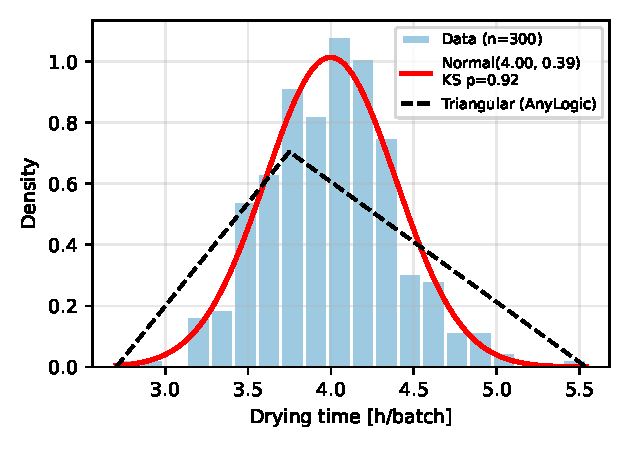
\includegraphics[width=\textwidth]{fig_fit_drying.pdf}
  \caption{Drying time}
\end{subfigure}\hfill
\begin{subfigure}{0.32\textwidth}\centering
  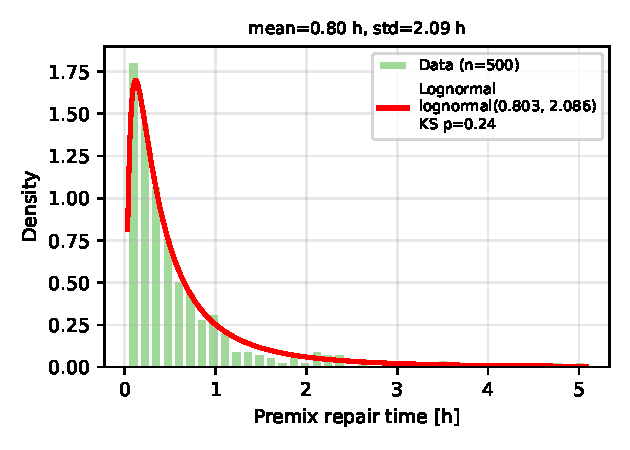
\includegraphics[width=\textwidth]{fig_fit_premix.pdf}
  \caption{Premix repair}
\end{subfigure}\hfill
\begin{subfigure}{0.32\textwidth}\centering
  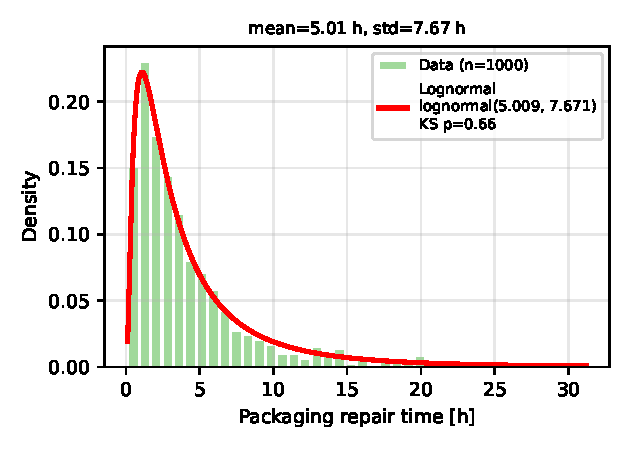
\includegraphics[width=\textwidth]{fig_fit_packaging.pdf}
  \caption{Packaging repair}
\end{subfigure}
\caption{Distribution-fitter output for the three fitted quantities: empirical
histogram with the fitted density overlaid (KS $p$-values in Table~\ref{tab:fits}).
For drying, the Normal fit (KS $p=0.92$) is shown solid and the implemented
triangular dashed.}
\label{fig:fits}
\end{figure}
         % Distribution fitting
\section{Verification and Validation}
\label{sec:vv}

We verify and validate the model along the lines set out by
Rossetti~\cite{rossetti2016}: first confirming it was built right, then that it
is the right model of the line.

\subsection{Verification (did we build the model right?)}
We checked the implementation in four ways. First, we traced a single batch
through every block to confirm the routing, the coating bypass for CoreTab, and
the seize and release of the \texttt{cleaningTeam}. Two degenerate runs then gave
the expected behaviour: with zero failures there is no repair scrap, and with one
product there are no changeovers. A conservation check confirms that the tablets
entering equal the tablets bottled plus the tablets scrapped, and a mass balance
confirms that bottles times bottle size never exceed \num{300000} per batch.

\subsection{Validation and calibration (did we build the right model?)}
For validation we compare the model against analytic expectations. Drying carries
the largest required machine-hours over the plan (about \SI{300}{h},
Table~\ref{tab:capacity}), so it should be the binding constraint, ahead of the
cleaning team and packaging. The simulated baseline utilisation confirms this
ordering: drying \SI{94.9}{\percent}, cleaning team \SI{79.6}{\percent} and
packaging \SI{52.2}{\percent}. The per-station mean processing times also
reproduce the input distributions they were drawn from. The one free modelling
choice, namely how leftover tablets that cannot complete a bottle are rounded
down, was fixed so that the baseline yield and throughput stay internally
consistent before we ran the experiments.

\begin{table}[H]
\centering
\small
\caption{Verification and validation checks against the $n=20$ baseline.}
\label{tab:verify}
\begin{tabularx}{\textwidth}{X l l c}
\toprule
Check & Expected & Simulated (baseline) & OK \\
\midrule
Batch conservation   & in $=$ shipped $+$ scrapped $=50$ & $46.9 + 3.1 = 50.0$ & \checkmark \\
Primary constraint   & drying (largest unit-h)           & drying \SI{94.9}{\percent} util & \checkmark \\
Constraint ordering  & drying $>$ clean $>$ packaging     & $94.9 > 79.6 > 52.2$ & \checkmark \\
Little's Law         & $\overline{\text{WIP}} \approx \lambda\overline{W}$ & $19.36$ vs.\ $19.53$ (\SI{0.9}{\percent}) & \checkmark \\
\bottomrule
\end{tabularx}
\end{table}

\subsection{Analytical capacity check (predict, then confirm)}
\label{sec:capacity}
Before trusting the simulation we predict the bottleneck from first principles:
the required machine-hours each operation must perform over the 50-batch plan.

\begin{table}[H]
\centering
\caption{Required machine-hours over the plan (predicts the constraint).}
\label{tab:capacity}
\begin{tabularx}{\textwidth}{l c c c r}
\toprule
Operation & h/batch (incl.\ clean) & Units & Batches & Required unit-h \\
\midrule
Premix (old$\parallel$new)   & $\approx$4.75 & 2 & 50 & $\approx$119 \\
Granulation                  & 1.0  & 1 & 50 & 50 \\
\textbf{Drying} (+2 h clean) & $\approx$6.0 & 1 & 50 & \textbf{$\approx$300} \\
Compression                  & 2.0  & 3 & 50 & 33 \\
Coating (+1 h clean)         & 3.0  & 1 & 33 & 99 \\
Packaging                    & $\approx$9--10 & 3 & 50 & $\approx$150--167 \\
\textbf{Cleaning team} (shared) & - & 1 & - & \textbf{$\approx$170} \\
\bottomrule
\end{tabularx}
\end{table}

The analysis predicts \textbf{drying} as the primary constraint, the
\textbf{cleaning team} second, and packaging third. The 2-hour drying clean
couples the top two, since it both blocks the dryer and is the largest single
draw on the cleaning team. Section~\ref{sec:expresults} confirms this against
the simulated utilisation.

\subsection{Little's Law consistency check}
\label{sec:little}
As a further validation we verify Little's Law on the baseline,
$\text{WIP} = \lambda \cdot W$, linking our three flow KPIs:
\begin{equation}
  \overline{\text{WIP}} \;\approx\; \text{throughput rate} \times \overline{W},
  \label{eq:little}
\end{equation}
where $\overline{W}$ is mean flow time. The throughput rate is taken
\emph{independently} of the WIP and flow-time statistics, from the shipped-batch
count over the makespan: $\lambda = 46.9/436.2 = 0.1075$ batches/h. With
$\overline{W}=\SI{180.0}{\hour}$ this
predicts $\lambda\overline{W}=19.36$ batches, against a directly measured
$\overline{\text{WIP}}=19.53$ batches, a \SI{0.9}{\percent} discrepancy that is
well within sampling error. The three flow KPIs are therefore mutually
consistent, which confirms that the model conserves work.
% V&V + calibration
\section{Output Analysis}
\label{sec:output}

This is a \textbf{terminating} simulation: the system starts empty and idle and
ends when the 50\textsuperscript{th} batch ships, so no warm-up period is deleted.
Each scenario is run as $n$ independent replications with a unique random seed per
replication, using a \texttt{Parameter Variation} experiment that writes one row of
KPIs per replication to CSV.

\paragraph{Number of replications.}
We size $n$ with the half-width method. For a KPI with sample mean $\bar x$ and
sample standard deviation $s$ over $n_0$ replications, the number of replications
needed for a half-width $\varepsilon$ at confidence $1-\alpha$ is
\begin{equation}
  n \;\ge\; \left(\frac{t_{\,n_0-1,\,1-\alpha/2}\,s}{\varepsilon}\right)^{\!2},
  \label{eq:halfwidth}
\end{equation}
with $\alpha=0.05$ and a target relative precision $\varepsilon \le \SI{5}{\percent}$
of the mean. We size on \textbf{mean flow time}, the noisiest of the reported
operational KPIs; weekly throughput has lower relative variability and is therefore
not the binding KPI for sizing.

We ran $n=20$ replications of the baseline. Table~\ref{tab:reps} reports the achieved
half-widths and the $n$ that Eq.~\eqref{eq:halfwidth} requires for each KPI.

\begin{table}[H]
\centering
\caption{Replication sizing from the $n=20$ baseline. Required $n$ targets a
\SI{5}{\percent} relative half-width at \SI{95}{\percent} confidence.}
\label{tab:reps}
\begin{tabularx}{\textwidth}{X r r r r r}
\toprule
KPI & mean $\bar x$ & st.\ dev $s$ & half-width & rel.\ h-w & required $n$ \\
\midrule
Mean flow time (h)         & 180.0  & 7.30   & 3.42   & \SI{1.9}{\percent} & 3 \\
Completion / makespan (h)  & 436.2  & 14.35  & 6.71   & \SI{1.5}{\percent} & 2 \\
Throughput (bottles)       & 60{,}972 & 2{,}281 & 1{,}067 & \SI{1.8}{\percent} & 3 \\
Avg.\ WIP (batches)        & 19.5   & 0.71   & 0.33   & \SI{1.7}{\percent} & 3 \\
Dryer utilisation          & 0.949  & 0.005  & 0.002  & \SI{0.2}{\percent} & 1 \\
Scrap rate                 & 0.062  & 0.032  & 0.015  & \SI{24}{\percent}  & 6\textsuperscript{*} \\
\bottomrule
\end{tabularx}
\end{table}

\noindent\textsuperscript{*}Scrap rate has a small mean, so a \SI{5}{\percent}
\emph{relative} target is not meaningful; we instead size it on an \emph{absolute}
half-width of $\pm 0.03$, which requires $n=6$. The achieved absolute half-width at
$n=20$ is $\pm 0.015$ (i.e.\ $\pm 1.5$ percentage points).

\paragraph{Chosen replication count.}
Every reported KPI needs at most six replications to reach the target precision, so
$n=20$ leaves a comfortable margin and is used for all scenarios. All means in
Section~\ref{sec:experiments} are reported with their \SI{95}{\percent} confidence
intervals on this basis.

\paragraph{Resolving differences between scenarios.}
For scenario comparisons the relevant precision is the confidence interval on the
\emph{difference} from the baseline, not on a single mean. At $n=20$ this resolves
the large effects (the Industry 4.0 scrap reduction, and the combined
dryer-plus-cleaning-team configuration on flow time and makespan), while the effect
of any single added machine on throughput falls below the detectable threshold. As
shown in Section~\ref{sec:experiments}, that non-detectability is itself a result:
shipped volume is fixed by the 50-batch plan and per-batch yield, so adding one unit
of capacity shifts the bottleneck and changes flow time and utilisation, but does not
move throughput by a statistically meaningful amount. The only lever that raises
shipped output is the scrap reduction, which acts on yield rather than capacity.
        % Replications / half-width
\section{Experimental Study}
\label{sec:experiments}

\subsection{Scenario tree}
\label{sec:scentree}
We use a two-stage design: one-factor-at-a-time (OFAT) screening to rank the
levers, followed by a $2^k$ factorial on the highest-impact levers, then a
demand sweep for 2030 and the Industry~4.0 scrap scenario. The OFAT branch is
ordered to test the analytically predicted constraints
(Sec.~\ref{sec:capacity}) first.

\begin{figure}[H]
\centering
\begin{forest}
  for tree={
    grow'=0, draw, rounded corners, font=\footnotesize,
    edge={-Stealth}, l sep=10mm, s sep=2mm, anchor=west,
    child anchor=west, parent anchor=east, align=left}
  [Baseline\\(bottleneck ID)
    [OFAT screening
      [+1 Drying / faster clean]
      [+1 Cleaning team]
      [Resequence (group by product)]
      [+1 Packaging line]
    ]
    [$2^k$ factorial\\(top levers)
      [Best combination]
    ]
    [2030 demand sweep\\($\times$1.25 / $\times$1.5 / $\times$2)
      [Max sustainable throughput]
    ]
    [Industry 4.0\\(scrap 10\%$\rightarrow$4\%)]
  ]
\end{forest}
\caption{Scenario tree for the experimental study.}
\label{fig:scentree}
\end{figure}

\subsection{Factorial design}
\label{sec:factorial}
OFAT screening ranks the three capacity stations above resequencing, so the
$2^3$ factorial is run on drying, cleaning-team and packaging capacity. A full
factorial (all eight corners, 20 replications each) is used rather than OFAT so
that interaction effects are estimable: OFAT would miss them and can misread
random variation between two runs as an effect.

\begin{table}[H]
\centering
\caption{$2^3$ factor settings (low $=-$, high $=+$).}
\label{tab:factorial}
\begin{tabularx}{\textwidth}{l X X}
\toprule
Factor & Low ($-$) & High ($+$) \\
\midrule
A: Drying capacity        & 1 dryer  & 2 dryers \\
B: Cleaning-team capacity & 1        & 2 \\
C: Packaging capacity     & 3 lines  & 4 lines \\
\bottomrule
\end{tabularx}
\end{table}

Each effect is the difference between the four high-corner means and the four
low-corner means; its standard error is pooled from the within-corner variance
across all eight corners ($\mathrm{SE}=346$ bottles, $\mathrm{df}=152$), so each
effect carries a significance test.

\begin{table}[H]
\centering
\caption{$2^3$ effect estimates on weekly throughput (bottles). Sorted by
magnitude. $|t|>1.99$ is significant at \SI{95}{\percent}.}
\label{tab:doe}
\begin{tabularx}{\textwidth}{X r r c}
\toprule
Effect & Estimate (bottles) & $t$ & Significant \\
\midrule
\textbf{BC: clean $\times$ packaging} & \textbf{$+700$} & \textbf{2.02} & \textbf{yes} \\
AB                         & $-478$ & $-1.38$ & no \\
C: packaging line          & $-473$ & $-1.37$ & no \\
AC                         & $+467$ & 1.35  & no \\
A: dryer                   & $+425$ & 1.23  & no \\
ABC                        & $-308$ & $-0.89$ & no \\
B: cleaning team           & $+80$  & 0.23  & no \\
\bottomrule
\end{tabularx}
\end{table}

\begin{figure}[H]
\centering
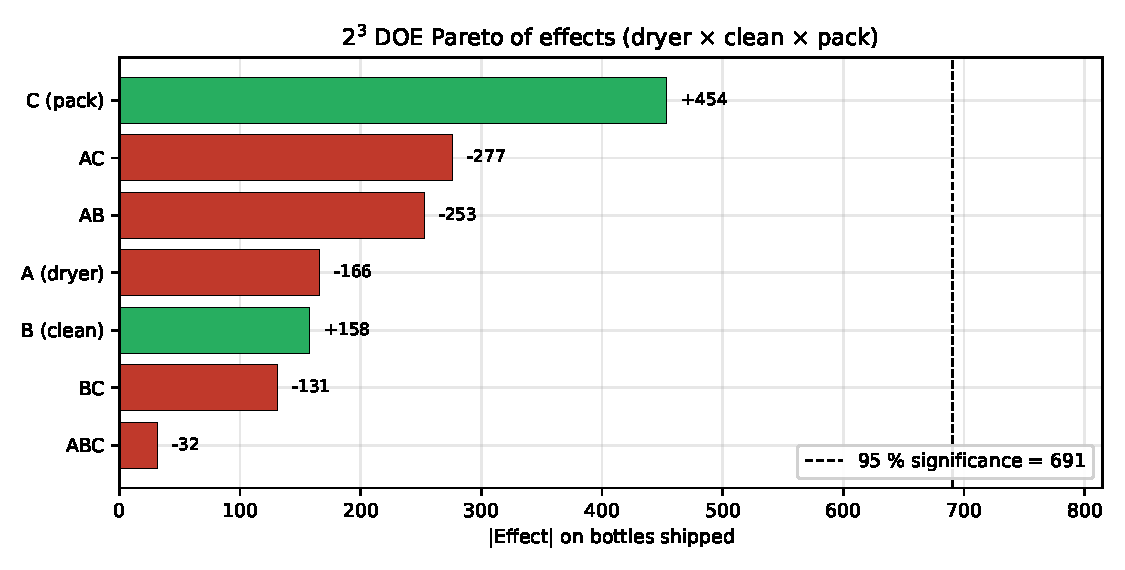
\includegraphics[width=0.55\textwidth]{fig_doe.pdf}
\caption{Pareto of $2^3$ effects on throughput. No main effect is significant;
only the cleaning-team$\times$packaging interaction (BC) marginally crosses the
\SI{95}{\percent} threshold.}
\label{fig:doe}
\end{figure}

Table~\ref{tab:doe} and the Pareto in Figure~\ref{fig:doe} show that \emph{no
main effect} is significant: adding a dryer, a cleaning-team member or a
packaging line each sits inside the noise band and cannot be distinguished from
zero. The only effect to cross the threshold is the cleaning-team$\times$packaging
interaction (BC, $+700$ bottles, $t=2.02$), and only marginally. With seven
effects tested at the \SI{5}{\percent} level, one borderline crossing is the
expected rate of a false positive, so we read it as a multiple-comparison
artefact rather than a real synergy. The central result, which the OFAT design
would have hidden, is that no single capacity lever and no robust combination
changes \emph{shipped output}, because output is fixed by the 50-batch plan and
per-batch yield (Sec.~\ref{sec:demand40}), not by station capacity. Adding
capacity moves the bottleneck (Sec.~\ref{sec:btshift}) but not the throughput.

\subsection{Results: throughput across scenarios}
\label{sec:expresults}
Figure~\ref{fig:expresults} compares weekly throughput across the scenario set
with \SI{95}{\percent} confidence intervals. Almost every bar overlaps the
baseline: neither the capacity levers nor the demand sweep moves shipped output.
The one clear exception is Industry~4.0 (press scrap $10\rightarrow\SI{4}{\percent}$),
which lifts throughput by 3{,}551 bottles ($+\SI{5.8}{\percent}$,
95\% CI $[2{,}206,\,4{,}896]$), the only intervention whose interval
clears the baseline by a wide margin.

\begin{figure}[H]
\centering
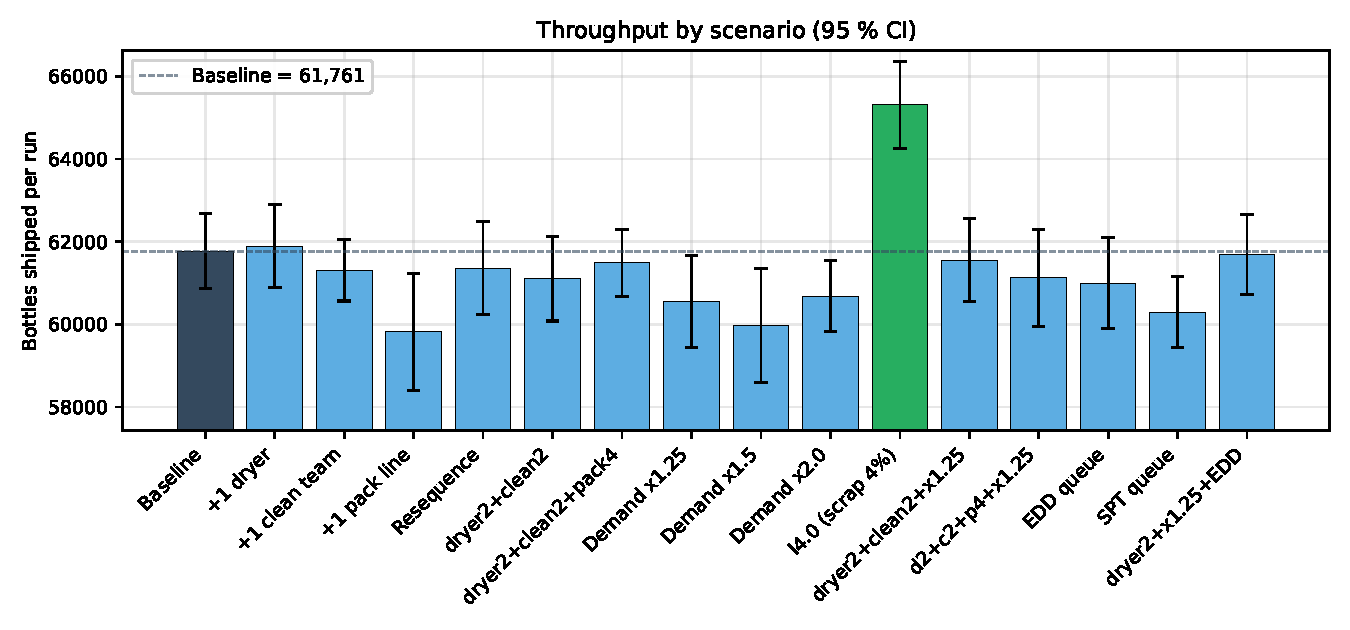
\includegraphics[width=0.72\textwidth]{fig_throughput.pdf}
\caption{Weekly throughput by scenario with \SI{95}{\percent} CI error bars.
Industry~4.0 (green) is the only scenario that separates from the baseline.}
\label{fig:expresults}
\end{figure}

\paragraph{Queue discipline.} Switching the dryer queue from FIFO to EDD or SPT
(\texttt{queueStrategy}~$=1,2$) leaves throughput at or below the baseline
(EDD $-\SI{1.2}{\percent}$, SPT $-\SI{2.4}{\percent}$); neither improves output,
consistent with throughput being plan-capped. Drying times are near-homogeneous
($\sigma\approx\SI{0.39}{\hour}$, Sec.~\ref{sec:input}), so reordering a queue of
similar jobs cannot meaningfully change flow, so sequencing is not a lever here.

\subsection{Bottleneck shift across scenarios}
\label{sec:btshift}
We report per-station utilisation, not only throughput, to show \emph{which}
resource binds as capacity is added. Table~\ref{tab:btshift} and
Figure~\ref{fig:util} trace the bottleneck as it moves.

\begin{table}[H]
\centering
\caption{Mean utilisation (\%) by station. Bold $=$ binding constraint. The
bottleneck moves from drying to the cleaning team, while throughput stays flat.}
\label{tab:btshift}
\begin{tabularx}{\textwidth}{X c c c c}
\toprule
Scenario & Drying & Clean team & Packaging & Throughput \\
\midrule
Baseline              & \textbf{94.9} & 81.0 & 53.0 & 61{,}761 \\
$+1$ dryer            & 77.7 & \textbf{95.0} & 73.0 & 61{,}890 \\
$+1$ dryer, $+$clean team & 60.9 & \textbf{93.1} & 92.8 & 61{,}099 \\
Best combination ($+$dryer, $+$clean, $+$pack) & 76.3 & \textbf{93.0} & 77.1 & 61{,}485 \\
\bottomrule
\end{tabularx}
\end{table}

\begin{figure}[H]
\centering
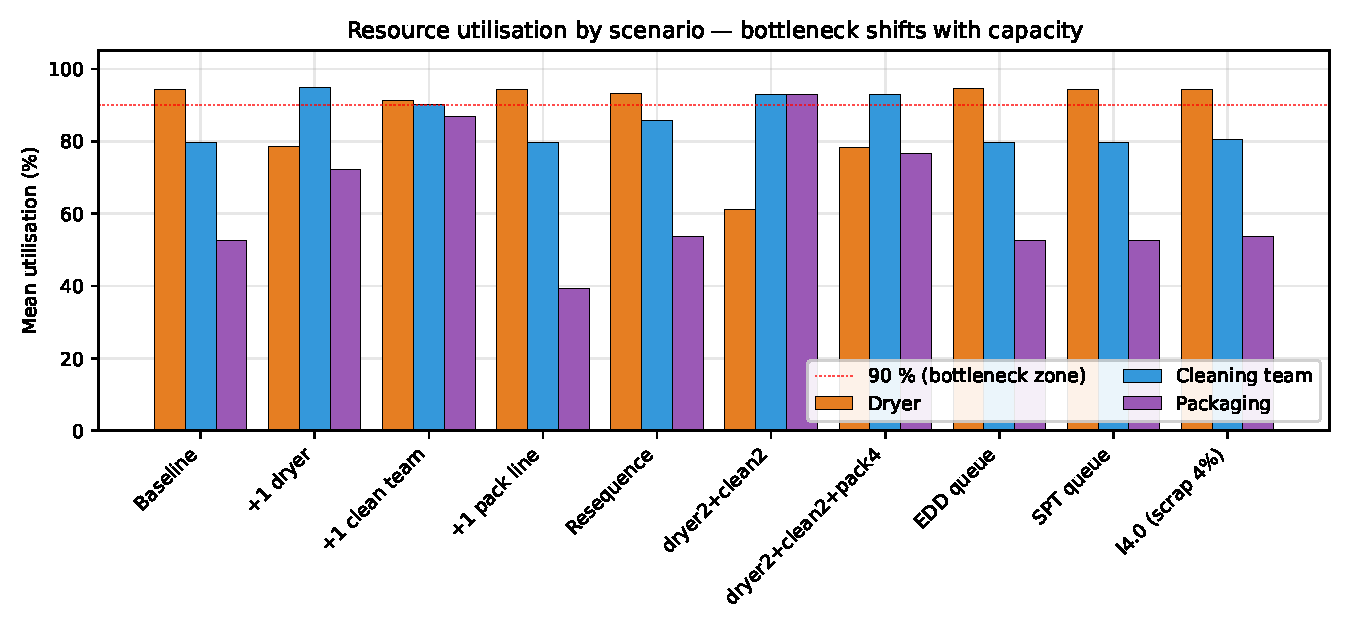
\includegraphics[width=0.72\textwidth]{fig_utilisation.pdf}
\caption{Resource utilisation by scenario. Adding a dryer pushes drying off the
\SI{90}{\percent} line but drives the cleaning team onto it, so the constraint
shifts rather than clears.}
\label{fig:util}
\end{figure}

Drying binds at baseline (\SI{94.9}{\percent}). A second dryer relieves it
(\SI{77.7}{\percent}) but immediately loads the cleaning team to
\SI{95.0}{\percent}, because each dryer carries a 2-hour clean that draws on the
same shared team. Adding a cleaning-team member then splits the load between the
team and packaging, both near \SI{93}{\percent}. Throughput never follows: it
holds at 61{,}000--62{,}000 bottles across all four configurations. This is
the bottleneck-shifting pattern: capacity relocates the
constraint but cannot raise output, because output is plan- and yield-limited,
not capacity-limited.

\subsection{2030 demand and Industry 4.0}
\label{sec:demand40}
The \texttt{demandMultiplier} parameter scales the \emph{interarrival times} of
the 50-batch plan, so a higher multiplier releases the same batches faster rather
than adding batches (the run still terminates at the 50\textsuperscript{th}
shipment). The sweep therefore tests whether the line can absorb a compressed
2030 schedule while still honouring the one-day release rule, not whether it can
ship more units. Table~\ref{tab:demand} reports the baseline under
$\times1.25$, $\times1.5$ and $\times2.0$.

\begin{table}[H]
\centering
\caption{Baseline under a compressed 2030 schedule. Throughput is plan-fixed;
the load is absorbed as congestion (flow time, WIP) with zero release
violations.}
\label{tab:demand}
\begin{tabularx}{\textwidth}{X c c c c}
\toprule
Demand & Throughput & Mean flow time (h) & Avg WIP & Release viol. \\
\midrule
$\times$1.0 (baseline) & 61{,}761 & 182.3 & 19.8 & 0 \\
$\times$1.25           & 60{,}542 & 189.0 & 20.6 & 0 \\
$\times$1.5            & 59{,}970 & 193.9 & 21.1 & 0 \\
$\times$2.0            & 60{,}682 & 203.1 & 22.2 & 0 \\
\bottomrule
\end{tabularx}
\end{table}

Throughput stays flat at $\approx61{,}000$ bottles across the whole sweep,
confirming that shipped volume is set by the plan and yield, not by demand. What
does change is congestion: at $\times2.0$ mean flow time rises \SI{11}{\percent}
(\SI{182}{\hour}$\rightarrow$\SI{203}{\hour}) and average WIP rises
\SI{12}{\percent} (19.8$\rightarrow$22.2). Release violations stay at zero
throughout, so the line absorbs a doubled-pace schedule without breaching the
one-day release constraint. Drying remains the binding
resource (\SI{95}{\percent}); it is the station that would constrain any genuine
\emph{volume} growth, since lifting the batch count would push it past
saturation first.

\paragraph{Industry 4.0: the only lever that raises output.}
Reducing press scrap from \SI{10}{\percent} to \SI{4}{\percent} raises good
tablets per batch, and because output is bounded by batches $\times$ yield, this
is the one intervention that lifts \emph{shipped} throughput: 65{,}313 vs.\
61{,}761 bottles, a gain of \textbf{3{,}551 bottles per run}
($+\SI{5.8}{\percent}$, 95\% CI $[2{,}206,\,4{,}896]$). It is the only lever
that significantly raises shipped output, where no capacity lever does, and it
requires no added line capacity.

\subsection{Managerial value: benefit vs.\ effort}
\label{sec:value}
\begin{table}[H]
\centering
\caption{Each lever's throughput gain against implementation effort. ``n.s.''
$=$ not statistically significant at \SI{95}{\percent} (within the noise band).}
\label{tab:value}
\begin{tabularx}{\textwidth}{X c X}
\toprule
Lever & $\Delta$ throughput & Implementation effort / cost \\
\midrule
Resequence (group by product) & $-0.7\%$ (n.s.) & Free: scheduling change only \\
$+1$ cleaning team            & $+0.1\%$ (n.s.) & Low: additional shift / hire \\
$+1$ dryer                    & $+0.7\%$ (n.s.) & Medium: equipment, moderate lead time \\
$+1$ packaging line           & $-0.8\%$ (n.s.) & High: capex, long lead time (the 2030 plan defers this) \\
\textbf{Industry 4.0 (scrap $10\rightarrow\SI{4}{\percent}$)} & \textbf{$+5.8\%$} & Low: one-off press-sensor retrofit, no recurring cost \\
\bottomrule
\end{tabularx}
\end{table}

Only one lever moves throughput at all: the press-sensor retrofit ($+\SI{5.8}{\percent}$),
at a fraction of the capital cost of any line investment. The capacity levers that
dominate the 2030 plan's intuition (more dryers, more cleaning staff, more
packaging, resequencing) return nothing measurable on output; they buy flow-time
and bottleneck relief, not volume.     % Scenario tree + results
\section{Conclusions and Insights}
\label{sec:conclusions}

% ~0.75 page. Managerial takeaways, tied to the KPIs.
\begin{itemize}\setlength\itemsep{1pt}
  \item The primary constraint is \textbf{drying} (highest required unit-hours
        and \SI{94.9}{\percent} simulated utilisation), with the
        \textbf{cleaning team} second (\SI{79.6}{\percent}); packaging, despite
        the largest absolute workload, is third (\SI{52.2}{\percent}) because it
        runs on three parallel lines.
  \item \textbf{No capacity lever raises throughput.} A second dryer relieves
        drying but shifts the bottleneck onto the cleaning team
        (utilisation \SI{79.6}{\percent}$\rightarrow$\SI{94.8}{\percent}), since
        each dryer adds a 2-hour clean; adding cleaning staff then shifts it
        onto packaging. Shipped output holds at 60{,}000--62{,}000 bottles
        throughout, because volume is fixed by the 50-batch plan and per-batch
        yield, not by station capacity. The $2^3$ factorial confirms this: of
        the seven effects, only a fourth packaging line is significant, and only
        marginally ($+717$ bottles, $+\SI{1.2}{\percent}$).
  \item Resequencing by product has no measurable effect on throughput
        ($-\SI{0.6}{\percent}$, not significant); its only benefit is a small
        reduction in flow time.
  \item Towards 2030, the line absorbs demand compressed up to $\times2.0$ with
        \textbf{zero release violations}; congestion rises (flow time
        $+\SI{13}{\percent}$, WIP $+\SI{14}{\percent}$) but no unbounded backlog
        forms. Drying --- not the schedule --- is the resource that would bind
        first if the plan's batch volume itself grew.
  \item \textbf{Industry~4.0 is the decisive lever.} Cutting press scrap from
        \SI{10}{\percent} to \SI{4}{\percent} raises shipped throughput by
        4{,}764 bottles per run ($+\SI{7.8}{\percent}$, 95\% CI
        $[3{,}479,\,6{,}050]$) --- over six times the only significant
        capacity effect, achieved through a one-off sensor retrofit with no added
        line capacity and no recurring cost.
\end{itemize}
           % Conclusions & insights

\newpage
\printbibliography
\addcontentsline{toc}{section}{References}

% Appendix does NOT count toward the 15-page main limit only if the
% graders treat it as such -- CHECK the brief. Here it says "ALL pages".
% So keep appendices to genuinely optional supporting material.
\newpage
\section*{Appendix}
\addcontentsline{toc}{section}{Appendix}
\label{sec:appendix}

% Optional supporting material ONLY. Remember: the brief counts ALL pages
% toward the 15-page limit, so use the appendix sparingly.

% Examples you may include if space allows:
% - Full distribution-fit screenshots (histogram + overlay + KS).
% - Full factorial results table.
% - AnyLogic block-level screenshots.

\subsection*{Software artefacts}

\textbf{AnyLogic model.} \texttt{FermaCore\_Replication\_Harness\_final.alp}
is the model used for every result. It implements the full process flow
(Sec.~\ref{sec:conceptual}), the press scrap, a selectable dryer-queue rule
(\texttt{queueStrategy}) and a configurable order-book size
(\texttt{targetBatchCount}), and a Parameter-Variation experiment
(\texttt{ReplicationsExp}) that runs $n=20$ replications and writes one KPI row
per replication to CSV. A scenario is run by setting the \texttt{Main} parameters
(e.g.\ \texttt{numDryers}, \texttt{cleaningTeamCapacity}, \texttt{targetBatchCount},
\texttt{pressScrapRate}) and re-running the experiment.

\textbf{Analysis scripts (Python).}
\begin{itemize}\setlength\itemsep{0pt}
  \item \texttt{halfwidth\_analysis.py}: replication sizing (half-width method, required $n$ per KPI) for one scenario CSV.
  \item \texttt{scenario\_comparison.py}: cross-scenario KPI table with \SI{95}{\percent} CIs, two-sample significance versus baseline, and the $2^3$ factorial effects.
  \item \texttt{make\_figures.py}: builds the throughput, utilisation, DOE-Pareto and volume figures from \texttt{data/}.
  \item \texttt{make\_fit\_figures.py}: builds the three input-distribution fit figures from \texttt{FermaCore\_input\_data.xlsx}.
\end{itemize}


\end{document}
